%%%%%%%%%%%%%%%%%%%%%%%%%%%%%%%%%%%%%%%%%%%%%%%%%%%%%%%%%%%%%%%%%%%%%%%%%%%%%%%%
%%% Homework Three -- Latex Template:
%%% Tested against the pdflatex compiler
%%%

\documentclass[english]{article}

%%%%%%%%%%%%%%%%%%%%%%%%%%%%%%%%%%%%%%%%%%%%%%%%%%%%%%%%%%%%%%%%%%%%%%%%%%%%%%%%
%%% Document Preamble
%%% - contains the external content (packages) and formatting settings
%%% - modification should be unnecessary unless you want to add additional
%%%   functionality or change the aesthetics

%%% Hyperref: insert links
% See: https://www.overleaf.com/learn/latex/Hyperlinks
\usepackage[unicode=true]{hyperref}

%%% Hyperref: links should appear blue as you would expect
\hypersetup{
  colorlinks=true,
  linkcolor=blue,
  urlcolor=blue,
  filecolor=blue,
}

%%% Listings: use to include code in your solutions
% See: https://www.overleaf.com/learn/latex/Code_listing
\usepackage{listings}

%%% Listings: setup defaults for code formatting
\lstset{
  language={C++},
  frame=tb,
  numbers=left,
  numberstyle=\tiny,
  basicstyle=\small\sffamily,
  breaklines=true,
}

%%% GraphicX: insert images (e.g. screenshots) into the document
% See: https://www.overleaf.com/learn/latex/Inserting_Images
\usepackage{graphicx}

%%% Float: Allows the use of the H specifier in images to force them in place
\usepackage{float}


%%% Enumitem: alphabetic enumerations with improved syntax
% E.g.
% (a) ...
% (b) ...
\usepackage[shortlabels]{enumitem}


%%% AMS Math: access to math environments alike align
% Aligning: https://www.overleaf.com/learn/latex/Aligning_equations_with_amsmath 
\usepackage{amsmath}

% Additional options when using tables
\usepackage{array}

%%% Custom commands

\newcounter{problemi}
\setcounter{problemi}{1}

\newcommand*{\headfont}{\fontsize{1.1em}{1.0em}\selectfont}


\newcommand\problem[1]{
  \noindent{\headfont\\\theproblemi. #1}\\
  \stepcounter{problemi}\smallskip
}

\newcommand*{\code}[1]{\texttt{#1}}


\begin{document}

%%%%%%%%%%%%%%%%%%%%%%%%%%%%%%% COVER PAGE %%%%%%%%%%%%%%%%%%%%%%%%%%%%%%%%%%%%%

\begin{centering}
    {\Large CSCE 221 Cover Page} \\ \medskip    
\end{centering}

Please list all sources in the table below including web pages which you used to solve or implement the current homework. If you fail to cite sources you can get a lower number of points or even zero, read more Aggie Honor System Office \url{https://aggiehonor.tamu.edu/} \\

% EDIT: the below information appropriately
\noindent
\begin{center}
    {\large
    \begin{tabular}{|p{0.35\linewidth}|p{0.45\linewidth}|} \hline
        Name          & Your Name         \\ \hline
        UIN           & 123456789         \\ \hline
        Email address & you@tamu.edu      \\ \hline
    \end{tabular}
    }
\end{center}

Cite your sources using the table below. Interactions with TAs and resources presented in lecture do not have to be cited. Please remove any sources you did not use.
\noindent
\begin{center}
    {\large
    \begin{tabular}{|>{\centering\arraybackslash}m{0.25\linewidth}|m{0.70\textwidth}|} \hline
        {\large People}            &
            \begin{enumerate}
                % EDIT
                % People: Add sources below as items
                \item Grigori Rasputin
            \end{enumerate}
        \\ \hline
        {\large Webpages}          & 
            \begin{enumerate}
                % EDIT
                % Webpages: Add sources below as items
                \item \url{ https://doi.org/10.1901/jaba.1974.7-497a}
            \end{enumerate}
        \\ \hline
        {\large Printed Materials} &
            \begin{enumerate}
                % EDIT
                % Printed Material: Add sources below as items
                \item None
            \end{enumerate}
        \\ \hline
        {\large Other Sources}     &
            \begin{enumerate}
                % EDIT
                % Other sources: Add sources below as items
                \item None
            \end{enumerate}
        \\ \hline
    \end{tabular}
    }
\end{center}

\pagebreak

%%%%%%%%%%%%%%%%%%%%%%%%%%%%%%% HOMEWORK TWO %%%%%%%%%%%%%%%%%%%%%%%%%%%%%%%%%%%%%

\begin{centering}
    {\Huge Homework 3}\\ \bigskip
    {\Large Due April 27 at 11:59 PM}\\ \bigskip
\end{centering}

\textbf{Typeset your solutions to the homework problems preferably in \LaTeX or LyX.
See the class webpage for information about their installation and tutorials.}

%%%%%%%%%%%%%%%%%%%%%%%%%%%%%%%%% PROBLEM 1 %%%%%%%%%%%%%%%%%%%%%%%%%%%%%%%%%%%%%%%

\problem{(10 points)
An airport is developing a computer simulation of air-traffic control that handles events such as landings and takeoffs. Each event has a \emph{time-stamp} that denotes the time when the event occurs. The simulation program needs to efficiently perform the following two fundamental operations:
}
\begin{enumerate}
    \item Insert an event with a given time-stamp (that is, add a future event)
    \item Extract the event with a smallest time-stamp (that is, determine the next event to process)
\end{enumerate}

\bigskip

\begin{enumerate}[(a)]
    \item What data structure should be used to implement the above operations efficiently? Explain your reasoning. \label{enum:id_datastruct}
    
    
    \item Provide the big-O asymptotic complexity of inserting a time-stamp into the data structure identified in part \ref{enum:id_datastruct}
    
    
    \item Provide the big-O asymptotic complexity of extracting a time-stamp from the data structure identified in part \ref{enum:id_datastruct}
    
    
    
\end{enumerate}

\pagebreak

%%%%%%%%%%%%%%%%%%%%%%%%%%%%%%%%% PROBLEM 2 %%%%%%%%%%%%%%%%%%%%%%%%%%%%%%%%%%%%%%%

\problem{(10 points)
Draw a 17-entry hash table that results from the using the hash function: $h(k) = ((3k + 5) \mod 11)$ to hash the keys: 12, 44, 13, 88, 23, 94, 11, 39, 20, 16, 5. Assume collisions are handled using the double hashing method. The secondary hash function is given by $h_s(k) = (7 - (k \mod 7))$.
}

\bigskip

\noindent Provide the final state of the table below:

\begin{table}[H]
    \centering
    \begin{tabular}{|*{17}{c|}} \hline
    &  &  &  &  &  &  &  &  &  &  &  &  &  &  &  &  \\ \hline
    \end{tabular}
    \caption{Resulting Hash Table}
\end{table}

\noindent Provide a record of all indexes which are probed (locations where algorithm inserts or attempts to insert a key). Note when collisions occur: \bigskip

\noindent \code{insert(12)}: \smallskip

\noindent \code{insert(44)}: \smallskip

\noindent \code{insert(13)}: \smallskip

\noindent \code{insert(88)}: \smallskip

\noindent \code{insert(23)}: \smallskip

\noindent \code{insert(94)}: \smallskip

\noindent \code{insert(11)}: \smallskip

\noindent \code{insert(39)}: \smallskip

\noindent \code{insert(20)}: \smallskip

\noindent \code{insert(16)}: \smallskip

\noindent \code{insert(5)}:

\pagebreak

%%%%%%%%%%%%%%%%%%%%%%%%%%%%%%%%% PROBLEM 3 %%%%%%%%%%%%%%%%%%%%%%%%%%%%%%%%%%%%%%%

\problem{(15 points)
    A \emph{complete} graph is an undirected graph in which every pair of vertices are connected with an edge. Consider the following complete graph with $n = 6$ vertices.
}

\begin{figure}[H]
    \centering
    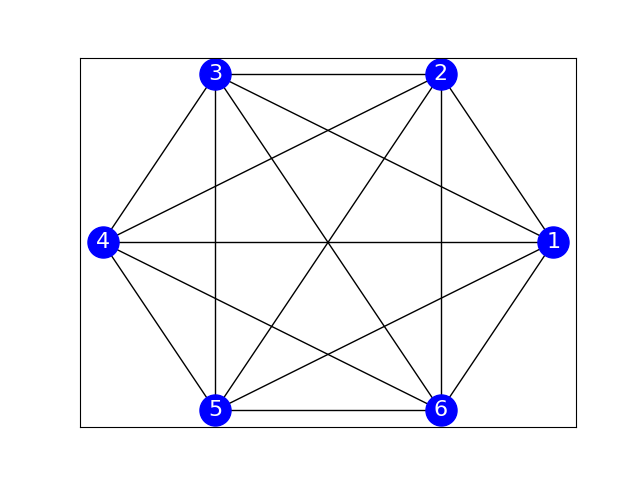
\includegraphics[width=0.6\textwidth]{complete_graph.png}
    \caption{A complete graph with $n = 6$ vertices}
    \label{fig:my_label}
\end{figure}

\begin{enumerate}[(a)]
    \item In what order does \code{DFS} explore vertices in the above graph? Assume \code{DFS} starts at vertex \code{4}. The adjacency lists are in ascending order by the numeric label.
    \item What is the running time of \code{DFS} on a complete graph with $n$ vertices? Provide an asymptotic big-oh bound in terms of the number of vertices. Explain your reasoning.
    \item How many back edges, forward edges, cross edges, and exploratory edges are generated by running \code{DFS} on a complete graph with $n$ vertices?
\end{enumerate}

\pagebreak

%%%%%%%%%%%%%%%%%%%%%%%%%%%%%%%%% PROBLEM 4 %%%%%%%%%%%%%%%%%%%%%%%%%%%%%%%%%%%%%%%

\problem{(10 points)
    Answer each of the following questions with a tight big-oh asymptotic bound. Justify with algorithmic reasoning.
}

\begin{enumerate}[(a)]
    \item A priority queue, \code{UnsortedMPQ}, is implemented based on an unsorted array. What is the running time of the operation which retrieves the minimum value?
    
    \begin{equation}
        \code{unsorted\_min(n)} \in O(\cdots)
    \end{equation}
    
    \item Dijkstra's algorithm is implemented based on this unsorted minimum priority queue. What is the running time of this implementation of Dijkstra's algorithm?
    
    \begin{equation}
        \code{dijkstra(V, E)} \in O(\cdots)
    \end{equation}
    
\end{enumerate}

\pagebreak

%%%%%%%%%%%%%%%%%%%%%%%%%%%%%%%%% PROBLEM 5 %%%%%%%%%%%%%%%%%%%%%%%%%%%%%%%%%%%%%%%

\problem{(15 points)
    Find the shortest path from D to all other vertices for the graph below.
}

\begin{figure}[H]
    \centering
    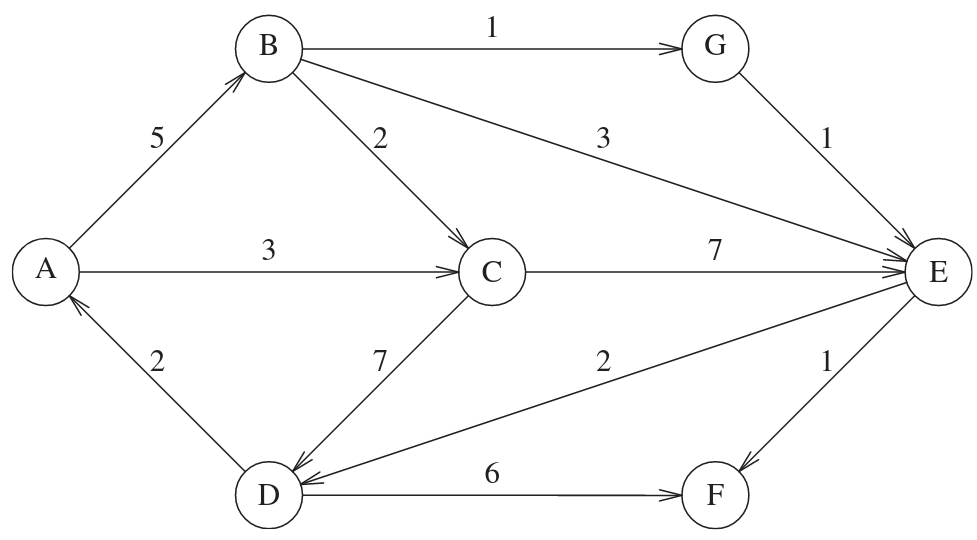
\includegraphics[width=0.8\textwidth]{dijkstras_graph.png}
\end{figure}

\begin{enumerate}[(a)]
    \item Illustrate the minimum priority queue at each iteration Dijkstra’s algorithm.
    
    % \begin{figure}[H]
    % \centering
    % 
\includegraphics[width=0.8\textwidth]{image.jpg}
    % \end{figure}
    
    \item Draw the Shortest Path Tree.
    
    % \begin{figure}[H]
    % \centering
    % 
\includegraphics[width=0.8\textwidth]{image.jpg}
    % \end{figure}
    
    \item What is the running time of the Dijkstra’s algorithm under the assumption that the graph is implemented based on an adjacency list and the minimum priority queue is implemented based on a binary heap?
    
    % \begin{equation}
    %     \code{dijkstra(V, E)} \in O(\cdots)
    % \end{equation}
    
\end{enumerate}

\pagebreak

%%%%%%%%%%%%%%%%%%%%%%%%%%%%%%%%% PROBLEM 6 %%%%%%%%%%%%%%%%%%%%%%%%%%%%%%%%%%%%%%%

\problem{(15 points)
    Find the shortest path from vertex 3 to all other vertices for the graph below.
}
\begin{figure}[H]
    \centering
    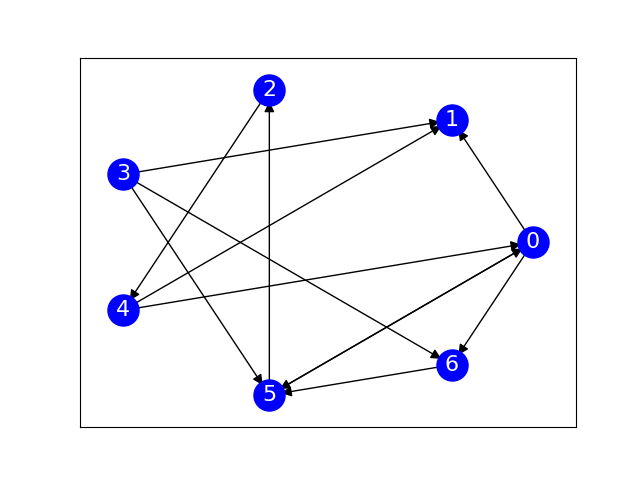
\includegraphics[width=0.8\textwidth]{./undirected.png}
\end{figure}

\begin{enumerate}[(a)]
    \item Which graph algorithm can solve the problem most \emph{efficiently}?
    \item Draw the Shortest Path Tree.
    
    % \begin{figure}[H]
    % \centering
    % 
\includegraphics[width=0.8\textwidth]{image.jpg}
    % \end{figure}
\end{enumerate}

\pagebreak

%%%%%%%%%%%%%%%%%%%%%%%%%%%%%%%%% PROBLEM 7 %%%%%%%%%%%%%%%%%%%%%%%%%%%%%%%%%%%%%%%

\problem{(10 points)
Apply the Dijkstra’s algorithm to find the shortest path from the vertex A to all the vertices in the graph below.
}
\begin{figure}[H]
    \centering
    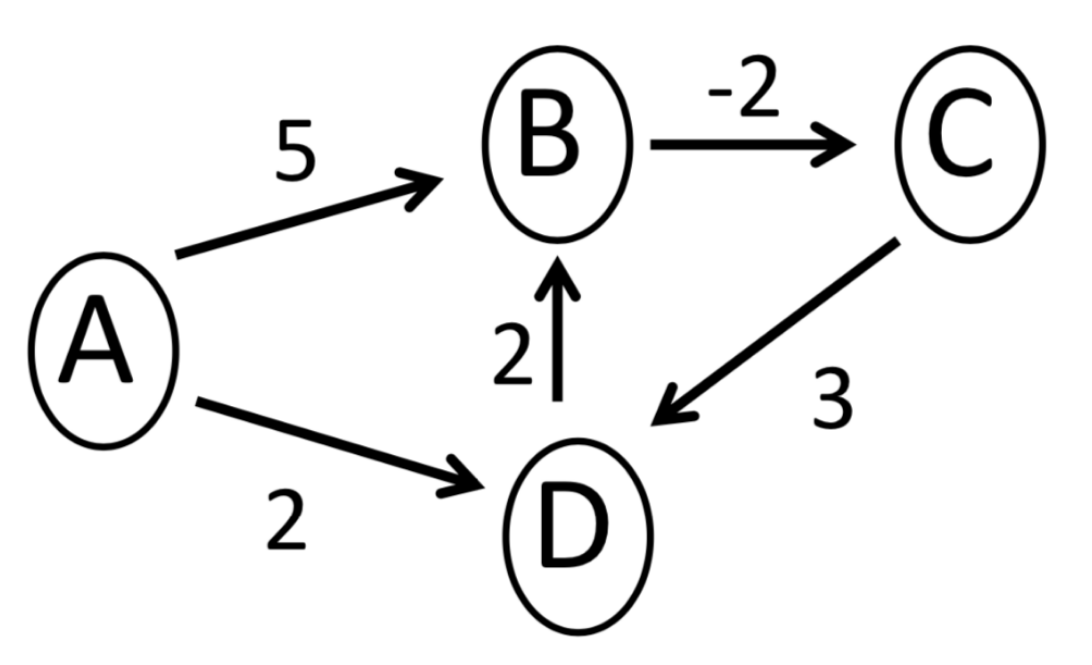
\includegraphics[width=0.6\textwidth]{p7_graph.png}
\end{figure}

\begin{enumerate}[(a)]
\item Illustrate  the  minimum  priority  queue  at  each  iteration  Dijkstra’s  algorithm.
    % \begin{figure}[H]
    % \centering
    % 
\includegraphics[width=0.8\textwidth]{image.jpg}
    % \end{figure}
\item Does the algorithm return the correct output?
\item Does Dijkstra's Theorem guarantee correctness for this graph? Explain.
\end{enumerate}

\pagebreak

%%%%%%%%%%%%%%%%%%%%%%%%%%%%%%%%% PROBLEM 8 %%%%%%%%%%%%%%%%%%%%%%%%%%%%%%%%%%%%%%%
\problem{(15 points) There are eight small island in a lake, and the state wants to build seven bridges to connect them so that each island can be reached from any other one via one or more bridges. The cost of bridge construction is proportional to its length. The distance between pairs of islands are given in the following table.
}

\begin{table}[H]
    \centering
    \begin{tabular}{ccccccccc}
          & 1 & 2   & 3   & 4   & 5   & 6   & 7   & 8   \tabularnewline
        1 & - & 240 & 210 & 340 & 280 & 200 & 345 & 120 \tabularnewline
        2 & - & -   & 265 & 175 & 215 & 180 & 185 & 155 \tabularnewline
        3 & - & -   & -   & 260 & 115 & 350 & 435 & 195 \tabularnewline
        4 & - & -   & -   & -   & 160 & 330 & 295 & 230 \tabularnewline
        5 & - & -   & -   & -   & -   & 360 & 400 & 170 \tabularnewline
        6 & - & -   & -   & -   & -   & -   & 175 & 205 \tabularnewline
        7 & - & -   & -   & -   & -   & -   & -   & 305 \tabularnewline
        8 & - & -   & -   & -   & -   & -   & -   & -   \tabularnewline
    \end{tabular}
    \caption{The distance between any two islands}
    \label{tab:my_label}
\end{table}


\begin{enumerate}
\item Illustrate the Prim's algorithm using the graph below. Draw the Minimum Spanning Tree. What is the length of the bridges?
    % \begin{figure}[H]
    % \centering
    % 
\includegraphics[width=0.8\textwidth]{image.jpg}
    % \end{figure}

\item Illustrate the Kruskal's algorithm using the graph below. Draw the Minimum Spanning Tree. What is the length of the bridges?
    % \begin{figure}[H]
    % \centering
    % 
\includegraphics[width=0.8\textwidth]{image.jpg}
    % \end{figure}

\end{enumerate}

\end{document}
